\begin{frame}{Diferencias divididas}
  \begin{exampleblock}{Cálculo eficiente de las diferencias divididas}
    \[
      f[x_0, \dots, x_k] = 
      \frac{f[x_1, \dots, x_k] - f[x_0, \dots, x_{k - 1}]}{x_k - x_0}
    \]
  \end{exampleblock}

  Para calcular un nuevo término, solo hace falta calcular \alert{una fila
  más de diferencias divididas}.
  
  \begin{center}
    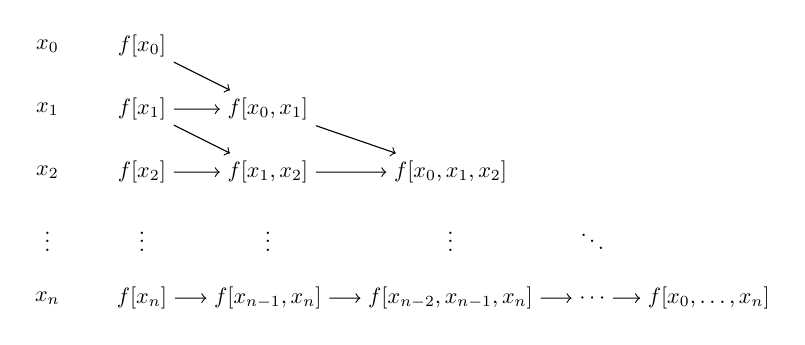
\begin{tikzpicture}[scale=0.8, transform shape]
      % Vector de x a la izda.
      \foreach \i in {0,1,2}
      {\node (\i) at (0,-\i) {$x_\i$};}
      \node (n) at (0,-4) {$x_n$};
      
      % Dots
      \node at (0,-3) {$\vdots$};
      \node at (1.5,-3) {$\vdots$};
      \node at (3.5,-3) {$\vdots$};
      \node at (6.4,-3) {$\vdots$};
      \node at (8.65,-3) {$\ddots$};
  
      %Nodes 1st column
      \foreach \y in {0,...,2}
      {\node (f1_\y) at (1.5,-\y) {$f[x_{\y}]$};}
  
      % Nodes 2nd column
      \foreach \y in {1,...,2}
      {\node (f2_\y) at (3.5,-\y) {$f[x_{\the\numexpr\y-1},x_{\the\numexpr\y}]$};}
  
      %Nodes 3rd column
      \node (f3_3) at (6.4,-2) {$f[x_0,x_1,x_2]$};
  
      %Nodes last row
      \node (f1_n) at (1.5,-4) {$f[x_n]$};
      \node (f2_n) at (3.5,-4) {$f[x_{n-1},x_n]$};
      \node (f3_n) at (6.4,-4) {$f[x_{n-2},x_{n-1},x_n]$};
      \node (dots) at (8.65,-4) {$\cdots$};
      \node (fn_n) at (10.5,-4) {$f[x_0,\dots,x_n]$};
  
      \draw[->] (f1_0) -- (f2_1);
      \draw[->] (f1_1) -- (f2_1);
      \draw[->] (f1_2) -- (f2_2);
      \draw[->] (f2_2) -- (f3_3);
      \draw[->] (f1_1) -- (f2_2);
      \draw[->] (f2_1) -- (f3_3);
  
      \draw[->] (f1_n) -- (f2_n);
      \draw[->] (f2_n) -- (f3_n);
  
      \draw[->] (f3_n) -- (dots);
      \draw[->] (dots) -- (fn_n);
    \end{tikzpicture}
  \end{center}
\end{frame}
